% Auriga starter — github:anishathalye/auriga, MIT.
%
% Engine: xelatex. beamerthemeauriga.sty loads fontspec unconditionally and
% hardcodes Raleway, Lato and Hack, none in the pinned compiler's font set.
% The vendored beamerthemeauriga.sty in this directory has all three swapped
% for Nimbus Sans (titles/body) and DejaVu Sans Mono (code) — see the comment
% in beamerthemeauriga.sty. Upstream's own README recommends building with
% LuaTeX via latexmk, but the theme has no LuaTeX-specific code (only
% \RequirePackage{fontspec}, identical under XeTeX); xelatex compiles it
% without issue.
\documentclass[14pt,aspectratio=169]{beamer}
\usepackage{tikz}

\usetheme{auriga}
\usecolortheme{auriga}

\definecolor{red}{RGB}{181, 23, 0}
\definecolor{blue}{RGB}{0, 118, 186}
\definecolor{gray}{RGB}{146, 146, 146}

\title{Zero-Downtime Schema Migrations at Scale}
\author{\underline{Priya Natarajan} \inst{1} \and Tomasz Kowalski \inst{1}}
\institute[shortinst]{\inst{1} Platform Engineering}

\begin{document}

{
  \setbeamercolor{page number in head/foot}{fg=white}
  \begin{frame}
    \titlepage
  \end{frame}
}

\begin{frame}{The problem}
  \begin{itemize}
    \item Schema changes on a live, high-write table used to mean a maintenance window
    \item Maintenance windows are a support burden and a trust problem
    \item Goal: change any column, index or constraint with zero downtime
  \end{itemize}
\end{frame}

\begin{frame}{Our approach}
  \begin{columns}
    \begin{column}{0.5\linewidth}
      \begin{itemize}
        \item Dual-write to old and new schema
        \item Backfill in bounded batches
        \item Verify with a checksum pass
        \item Cut over reads, then drop the old column
      \end{itemize}
    \end{column}
    \begin{column}{0.5\linewidth}
      \begin{figure}
        \centering
        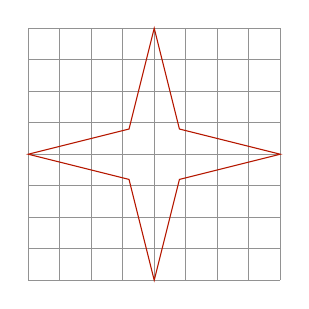
\begin{tikzpicture}[scale=1.6]
          \draw[step=0.25cm,color=gray] (-1,-1) grid (1,1);
          \draw[color=red] (1,0) -- (0.2,0.2) -- (0,1) -- (-0.2,0.2) -- (-1,0)
          -- (-0.2,-0.2) -- (0,-1) -- (0.2,-0.2) -- cycle;
        \end{tikzpicture}
        \caption{Four-phase rollout}
      \end{figure}
    \end{column}
  \end{columns}
\end{frame}

\begin{frame}[fragile]{Example: adding a NOT NULL column}
  \begin{verbatim}
ALTER TABLE orders ADD COLUMN region TEXT;
UPDATE orders SET region = 'unknown'
  WHERE region IS NULL LIMIT 5000;
-- repeat in batches, then:
ALTER TABLE orders ALTER COLUMN region
  SET NOT NULL;
  \end{verbatim}
\end{frame}

\begin{frame}{Results}
  \begin{itemize}
    \item 340+ migrations run with this pattern since rollout
    \item Zero maintenance windows in the last 14 months
    \item Median migration time down from 40 minutes to 6 minutes
  \end{itemize}
\end{frame}

\end{document}
